\chapter[Related works]{Related works}
\label{chapter:related_works}
% 다른 사람들의 관련 연구 소개
\section[LEO satellite FLSO schemes]{LEO satellite FLSO schemes}

\quad Mobility management for LEO satellite networks is actively being standardized within 3GPP. Whereas conventional TN possess a static topology, rendering explicit NG interface management procedures unnecessary, the high mobility of LEO satellites necessitates them. Consequently, procedures for NG interface management are actively being defined in 3GPP standards to support this dynamic connectivity [].
\begin{figure}[t]
  \centering
  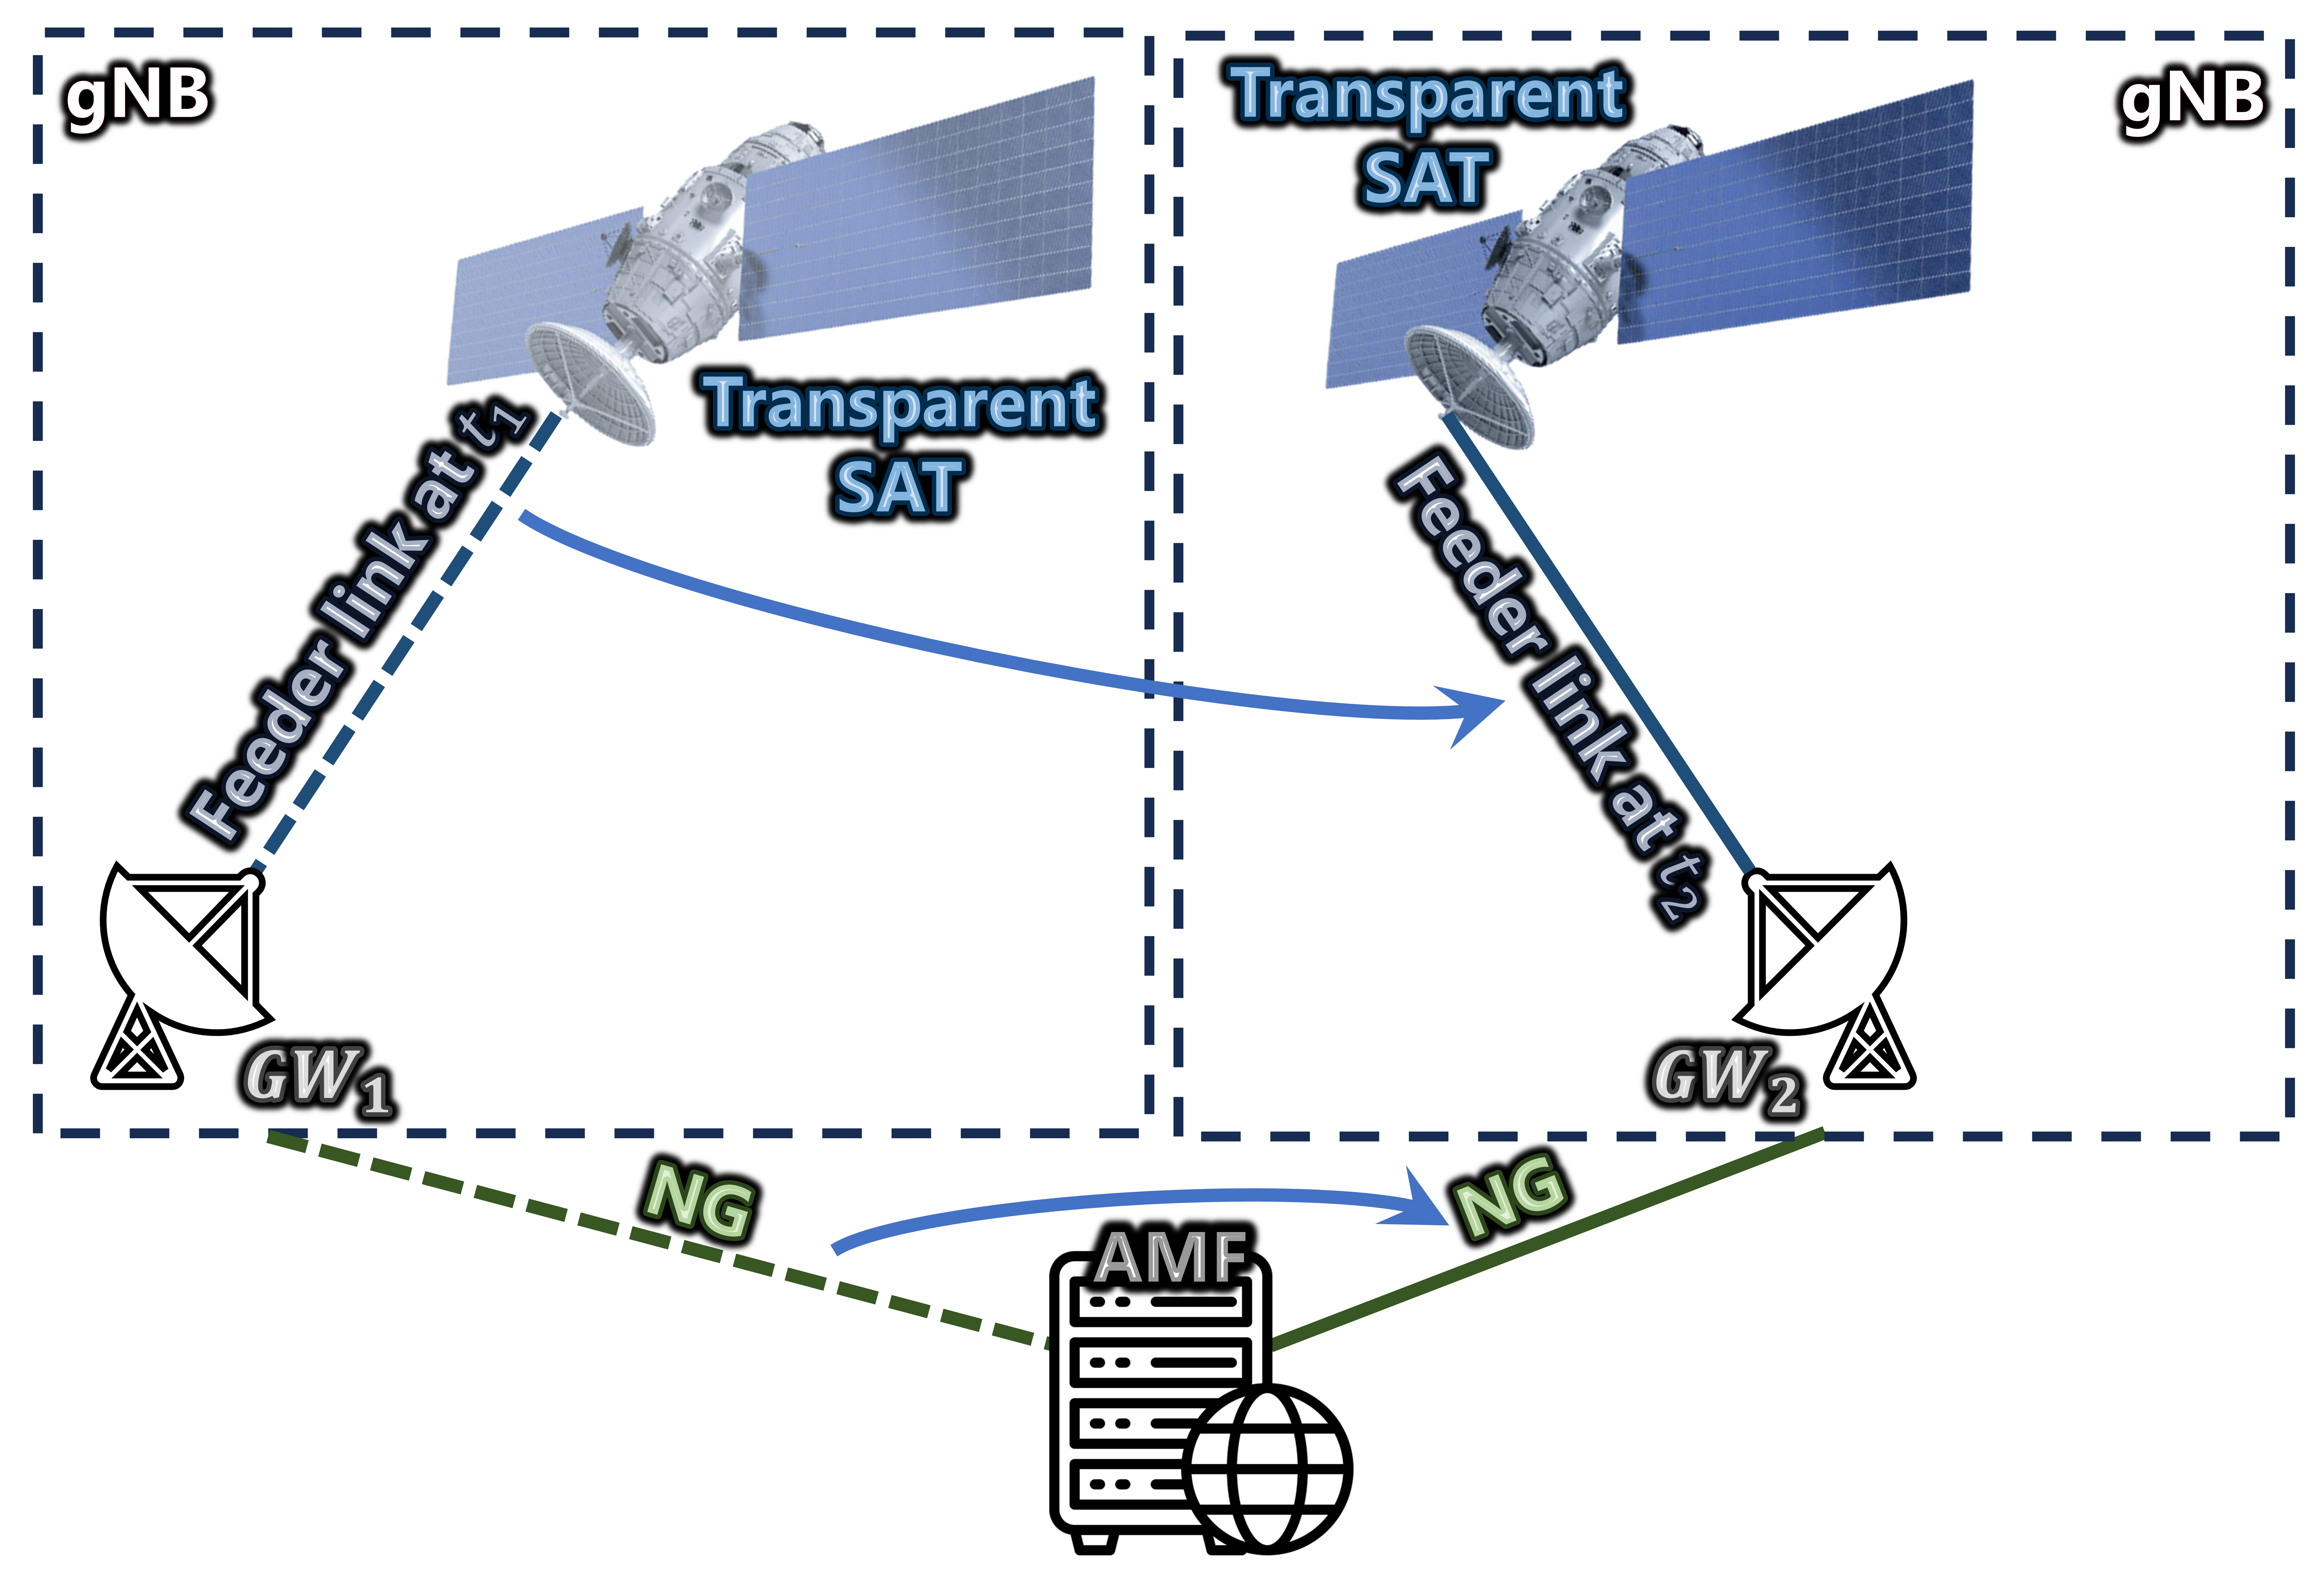
\includegraphics[width=1\linewidth]{figure/fig_sat_flso_trans.png}
  \caption{Feeder link architectures for transparent satellite}
  \label{fig:flso_arch_trans}
\end{figure}

\begin{figure}[t]
  \centering
  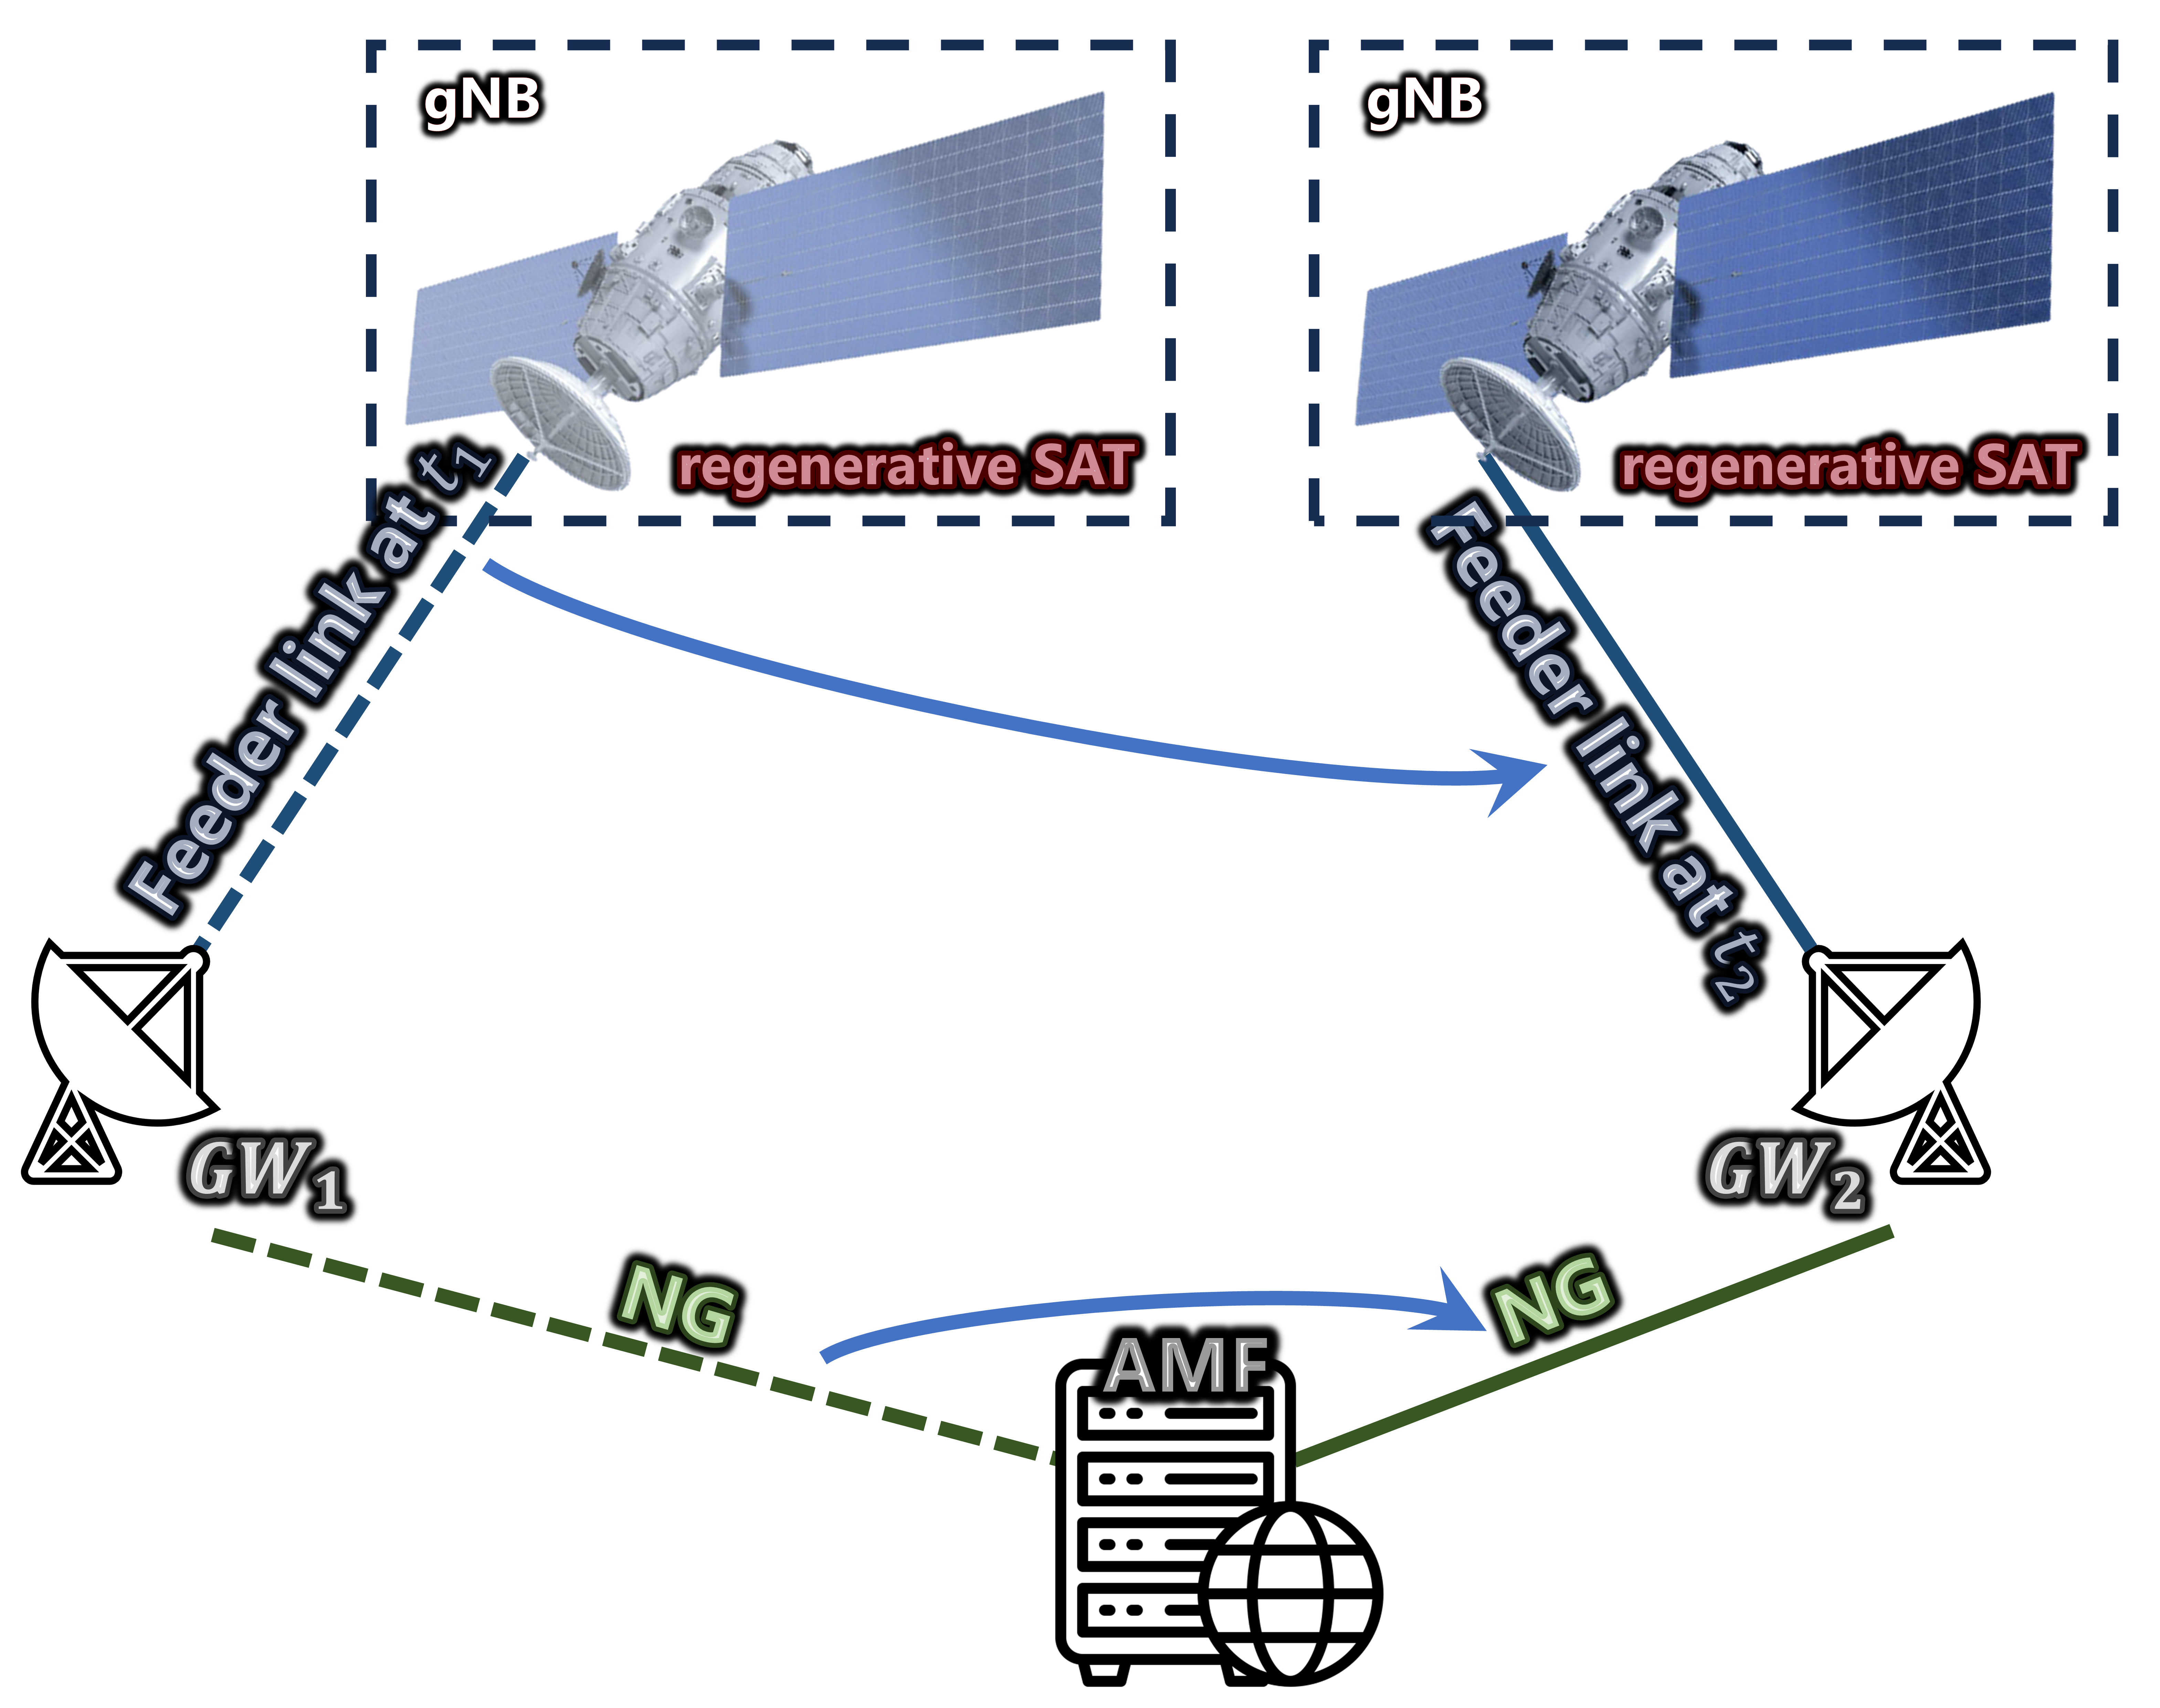
\includegraphics[width=1\linewidth]{figure/fig_sat_flso_reg.png}
  \caption{Feeder link architectures for regenerative satellite}
  \label{fig:flso_arch_reg}
\end{figure}
Furthermore, as shown in Fig. \ref{fig:flso_arch_trans}, the architecture impacts the HO process. For transparent satellites, the gNB is located at the ground GW and communicates with the UE via the service link. If the gNBs associated with different GWs are different, a FLSO induces a UE HO.
In contrast, as shown in Fig. \ref{fig:flso_arch_reg}, a regenerative satellite has an onboard gNB. This allows the UE to maintain its connection with the same gNB even during an FLSO; therefore, a UE HO does not occur as a direct result of the FLSO. Additionally, two FLSO methods exist. The first is hard FLSO, where the link is broken before the new one is established. The second is soft FLSO, where the transition occurs while the original link is maintained.
While 3GPP defines the architectures and mechanisms for executing an FLSO, the optimal selection policy—determining which available GW to switch to—is non-standardized and remains a critical challenge for network performance.
Related work addressing this selection problem has traditionally focused on simple heuristic strategies. These include signal-based methods selecting the GW with the strongest RSRP, distance-based methods selecting the closest GW.
However, these heuristic approaches are overly focused on link-level metrics like signal quality or stability at the moment of switching. They fail to consider the processing load and traffic distribution across the GW network. This omission leads to severe load imbalance, particularly in dense NTN scenarios where multiple satellites may select the same best GW simultaneously. This congestion at a single GW creates a bottleneck, degrading overall NTN backhaul efficiency and increasing latency, regardless of the satellite payload architecture.

% LEO 위성망의 이동성 관리는 3GPP에서 활발히 표준화되고 있습니다. 모든 위성은 ng 인터페이스로 게이트웨이와 amf/upf 코어망에 연결됩니다. 따라서 기존 지상망에서는 변화가 거의 없어서 NG 인터페이스의 관리 절차가 표준에 정의 되지 않았지만 LEO위성의 이동성을 위해 NG 인터페이스 관리 절차가 표준에서 정의중입니다 []. 또한 그림1과 같이 transparent 위성의 경우 gNB가 지상의 GW에 위치하고 서비스링크를 통해 UE와 통신하기 때문에 각 GW 간의 gNB가 다른 경우에는 FLSO 시 UE HO가 발생합니다. 반면, 그림 2와 같이 regenerative 위성은 gNB를 탑재하여 FLSO 시에도 UE는 동일한 gNB와 연결을 유지하므로 FLSO가 발생하더라도 UE HO가 발생하지 않습니다. 또한 피더링크 스위치오버 방식에도 두가지 방식이 있으며 먼저 연결이 끊고 다음 게이트웨이에 연결하는 하드 스위치오버 방식과 연결이 유지된 상태에서 게이트웨이를 전환하는 소프트 스위치오버 방식이 있습니다.



\section[Load Balancing in LEO Satellite Networks]{Load Balancing in LEO Satellite Networks}
\quad Load balancing in LEO NTN spans two tightly coupled planes: (i) the service-link plane, where beams/cells must be scheduled and powered to match spatio-temporal demand, and (ii) the feeder-link plane, where satellites select among candidate gateways (GWs) via FLSO to provision backhaul capacity. Overlapping satellite footprints and rapidly varying link conditions make naive single-metric selection fragile under realistic traffic and topology changes.
% LEO NTN의 로드 밸런싱은 (i) 빔/셀을 수요에 맞게 스케줄·전력할당하는 서비스 링크 면과,
% (ii) 위성이 FLSO를 통해 후보 GW 중에서 백홀을 선택하는 피더 링크 면의 두 차원에서 긴밀히 결합되어 수행됩니다.
% 위성 커버리지 중첩과 빠르게 변하는 링크 조건 때문에 단일 지표 기반의 단순 선택은 실제 트래픽/토폴로지 변화에 취약합니다.

\quad The coupling depends on payload architecture. In transparent payloads, changing the GW typically changes the serving gNB, so an FLSO may induce a UE HO; thus the policy must trade off radio-quality/ToS gains against HO cost and risk. In regenerative payloads, the UE remains attached to the on-board gNB across an FLSO, but backhaul congestion and path stretch still dominate end-to-end latency and reliability.
% 이 결합 정도는 페이로드 아키텍처에 달려 있습니다.
% 투명(transparent) 페이로드에서는 GW 변경이 보통 서비스 gNB 변경을 수반하므로 FLSO가 UE HO를 유발할 수 있어,
% 무선 품질/ToS 이득과 HO 비용·리스크 간의 절충이 필요합니다.
% 재생(regenerative) 페이로드에서는 UE가 탑재 gNB에 계속 부착되지만, 백홀 혼잡과 경로 증가가 종단 간 지연/신뢰성에 큰 영향을 줍니다.

\quad Practical constraints include finite GW processing/backhaul capacity, feeder-link spectrum/time constraints, visibility and elevation masks, and control-plane overhead. Excessive switchover induces thrashing; hard FLSO risks packet loss, whereas soft FLSO consumes duplicate backhaul resources during overlap. Effective policies therefore require hysteresis and cooldown to stabilize decisions.
% 실제 제약으로는 GW의 처리/백홀 용량 한계, 피더링크 자원 제약, 가시성·고도 마스크, 제어면 오버헤드 등이 있습니다.
% 과도한 스위치오버는 스래싱을 유발하며, 하드 FLSO는 패킷 유실 위험이, 소프트 FLSO는 겹침 구간 동안의 중복 자원 소비가 발생합니다.
% 따라서 안정화를 위한 히스테리시스와 쿨다운이 필요합니다.

\quad Representative objectives are: (1) maximize end-to-end throughput or minimize flow delay; (2) balance GW load (e.g., fairness across GWs) to avoid bottlenecks; (3) maintain radio quality (RSRP/SINR) and acceptable ToS; and (4) minimize switching costs, measured by FLSO frequency and, when applicable, UE HO count. Queue stability at GWs serves as an operational constraint.
% 대표 목표는 (1) 종단 간 처리량 최대화/지연 최소화, (2) 병목을 피하기 위한 GW 간 로드 밸런싱(공정성),
% (3) 무선 품질(RSRP/SINR)과 허용 가능한 ToS 유지, (4) FLSO 빈도와(해당 시) UE HO 횟수로 측정되는 스위칭 비용 최소화입니다.
% 또한 GW 큐 안정성은 운용 제약으로 고려됩니다.

\quad Heuristic baselines\textemdash strongest-RSRP, nearest-GW, fixed thresholds, or distance/time triggers\textemdash are simple but myopic, ignoring time-varying congestion and multi-satellite interactions. We instead target an adaptive policy: the state aggregates per-GW load, candidate link quality and ToS, recent FLSO history, and short-term visibility; the action selects a target GW (and can be extended to joint beam scheduling); the reward combines throughput/SINR and fairness, with penalties for overload and switching. Such a learning-based design anticipates congestion rather than merely reacting to it.
% RSRP 최대, 최근접 GW, 고정 임계값, 거리/시간 트리거 등 휴리스틱 기법은 단순하지만,
% 시간에 따라 변하는 혼잡과 다중 위성 상호작용을 간과하는 단견을 갖습니다.
% 본 연구는 적응형 정책을 지향합니다: 상태는 GW별 부하, 후보 링크 품질과 ToS, 최근 FLSO 이력, 단기 가시성 정보를 포함하고,
% 행위는 대상 GW 선택(확장 시 빔 스케줄링 결합)이며, 보상은 처리량/SINR과 공정성을 결합하고 과부하·스위칭에 패널티를 부여합니다.
% 이러한 학습 기반 설계는 단순 반응이 아닌 혼잡을 선제적으로 예견합니다.



%한상민 논문 12,14랑 LG cto 발표자료 확인해보기
%하나의 저궤도 위성이 운용할 수 있는 총 빔의 개수와 동시에 운용하는 빔 최대 개수를 각각 1,658개, 424개
%Multi-Satellite Beam Hopping Based on Load Balancing and Interference Avoidance for NGSO Satellite  Communication  System
%38.821 6.2.4에서는 추후 빔간 주파수 자원할당에 논의해야한다고 함
%링크 관리 문제는 현재 3GPP 표준에도 정의 되어 있듯이 빔 호핑을 사용하여 위성이 고정된 빔 대신 트래픽 수요가 있는 특정 지상 셀 영역에만 빔을 순차적으로 할당하는 기술도 논의되고 있다.
%빔 호핑에서 cell의 중앙을 기준으로 sinr을 계산하는 이유는 빔은 정해진 pci를 가지기 때문에 가장 sinr을 높게 빔을 설계하기 위해서임.
%따라서 PCI를 기준으로 빔 호핑 하는 논문을 찾아야함.